\documentclass[11pt]{article}
\usepackage[margin=1in]{geometry}
\usepackage{amsmath,amssymb}
\usepackage{graphicx}
\usepackage{booktabs}
\usepackage[hidelinks]{hyperref}
\usepackage{caption}
\captionsetup{font=small}

\title{\textbf{YHer: An Evidence-Bound Diagnostic Learning System for High-School Chemistry}\\
\large An Engineering Evidence Report}
\author{\textbf{Licheng Tu}\thanks{Independent researcher.}}
\date{September 2026}

\setlength{\emergencystretch}{3em}
\begin{document}
\makeatletter\@ifundefined{sec@limitations}{}{}\makeatother
\maketitle

\begin{abstract}
\noindent
We present YHer, a single-node diagnostic learning loop for Shanghai high-school chemistry built on one design constraint: every conclusion a student sees must be traceable to evidence that cannot be invented. Standard solutions are projected only from records that passed answer verification against official examination keys; the item bank is recovered from original examination Word documents rather than generated; resource recommendations carry signed provenance; and the browser never receives answers, rubrics, or item identities before a response is locked in. We report the engineering evidence for each of these claims. A data pipeline converts 6,083 raw sliced items from public Shanghai chemistry examinations into 3,329 structured items (block schema, formulas and figures preserved), from which a ten-batch usability audit selects 2,526 into a whitelist and 1,202 into service (47.6\%). Five blind rounds of AI question generation measure whether generated questions are distinguishable from real items: 87\% under adversarial comparison from scratch, 65\% overall for style transfer (60\% under fair conditions)---yielding a generation boundary that the product honors today. A three-round architecture audit (six literature lanes, three red-team passes, one independent verification round) returns 4 keep / 10 modify / 5 replace / 2 downgrade verdicts across twenty-one engine components, with the hardest finding that all hand-set constants in the engine lacked calibration evidence. \textbf{The manuscript is an engineering-evidence report. All conclusions are simulation-derived, audit-derived, or engineer-derived; there is no real-student validation. No claim herein rests on learner data.}
\end{abstract}

\section{Introduction}
\label{sec:intro}

\subsection{A concrete failure}
A student completes a five-item diagnostic session, all of them on the molarity of solutions. The system reports ``unstable reasoning''. The student asks: \emph{which answer led you there?} In most AI tutoring products in 2026, this question cannot be answered---not because the diagnosis is wrong, but because the diagnosis is not \emph{built} on a per-item trace. The language model produced a statement; the statement is not linked, by construction, to any particular response, to any particular standard answer, or to any particular source document.

In the Chinese gaokao system, the most valuable educational asset is not content: it is judgment. A student's question is rarely ``what is the answer to item 12?'' but ``why do I keep failing at this exact kind of step, and what do I do in the next ten minutes?'' A good teacher produces that judgment, and can always answer the follow-up question---with an answer book, a worked example, and a record of what the student actually submitted.

\subsection{The design constraint}
Our central design constraint is therefore not ``make the model smarter''. It is: \emph{make every answer a student sees traceable to something that cannot be invented}. We call this \textbf{evidence-binding}. Concretely, the design freezes:

\begin{itemize}\setlength{\itemsep}{0pt}\setlength{\parskip}{0pt}\setlength{\parsep}{0pt}
\item \textbf{Standard solutions} are projected only from records with \texttt{answer\_verification=passed}, whose provenance is an official answer key (Section~\ref{sec:data-pipeline}).
\item \textbf{The item bank} is derived from original examination Word documents via a deterministic extraction pipeline---not model-generated (Section~\ref{sec:data-pipeline}).
\item \textbf{Recommendations} carry a signed evidence trail (\path{track_map_v1.yaml} + \path{curriculum_runtime_v1.json}); unverified resources stay neutral (Section~\ref{sec:system}).
\item \textbf{The browser fails closed}: answers, rubrics, and item IDs are never delivered before the response is locked in (Section~\ref{sec:system}).
\end{itemize}

This is not a privacy filter layered on a model; it is a \emph{scoping decision}. The generative layer does limited selection and language organization. It cannot create new chemistry facts.

\subsection{Contributions}
We report the following, each quantified and each falsifiable:
\begin{enumerate}\setlength{\itemsep}{0pt}\setlength{\parskip}{0pt}\setlength{\parsep}{0pt}
\item \textbf{An end-to-end system} with a frozen three-family design (diagnostic / practice / held-out), four-state belief model, expected-information-gain item selection, signed recommendation, and replayable profile (Section~\ref{sec:system}).
\item \textbf{A data-pipeline methodology} that converts 6,083 raw slices from Shanghai chemistry examinations into 1,202 serviceable items---a 19.8\% end-to-end yield---with a ten-batch usability audit whose acceptance line is ``a student can use it'', not ``it renders'' (Section~\ref{sec:data-pipeline}).
\item \textbf{A measured generation boundary}: five blind rounds (total cost \textyen13.87) establish that from-scratch AI generation is distinguishable from real items at 87\% under adversarial pairwise comparison and is therefore confined to low-stakes practice slots; style transfer reaches 65\% distinguishability / 60\% fair-conditions and is alive (Section~\ref{sec:exp1}).
\item \textbf{An audit protocol} whose evolution itself is evidence: three rounds of component-wise adjudication, independent re-review, six literature lanes, and three red-team passes returning 4 keep / 10 modify / 5 replace / 2 downgrade across 21 engine components (Section~\ref{sec:exp2})---and an explicit statement of what is \emph{not} validated (Section~\ref{sec:limitations}).
\end{enumerate}

\subsection{Scope and honesty}
We chose the Engineering Evidence genre deliberately. The product has \emph{no real-student validation} as of this manuscript. Every number in this paper is either a measured property of code, of files, or of a documented audit; where a number comes from simulation or from an audit, we say so in the same sentence. We have not run a randomized controlled trial or a pilot with students; Section~\ref{sec:limitations} enumerates what that absence means for every claim.

\section{Background and Motivation}
\label{sec:background}

The Shanghai high-school chemistry examination is a high-stakes, single-subject, closed-form assessment. It has a distinctive public-data property: original papers, with answer keys, are public documents, and 155 distinct papers (\texttt{group\_key}s) are recoverable as Word or PDF sources. This makes a per-item evidence trail \emph{architecturally possible} in chemistry in a way that it is not for, say, essay-based subjects.

The dominant AI-tutoring paradigm in 2026 is generation-first: a language model produces an answer, a hint, a diagnosis, or a recommendation directly from its weights and context. This has demonstrated competence on textbook tasks (e.g., math word problems, code, exams) and is increasingly studied in education settings, including knowledge tracing from tutor-student dialogues \cite{llmkt2025}, and tutoring-system intelligence augmented by LLMs \cite{tutorLLM2024}. However, the paradigm has a structural property that matters for high-stakes diagnosis: \emph{its statements are not bound to evidence by construction}. Even when the model is right, it cannot answer the follow-up question.

Evidence-binding is the alternative: make the trace the first-class artifact. This has engineering consequences. Data quality stops being a preprocessing detail and becomes the product's core asset; auditability stops being a compliance feature and becomes a design requirement. The remainder of this paper reports what those consequences cost, and what they bought.


\begin{figure}[t]
\centering
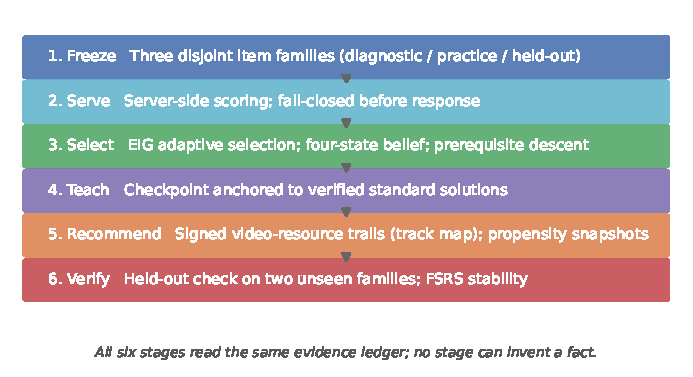
\includegraphics[width=\textwidth]{figures/fig1_system_flow.pdf}
\caption{Session flow. All six stages read from the same evidence ledger; no stage can invent a fact.}
\label{fig:flow}
\end{figure}
\section{System Design}
\label{sec:system}

Figure~\ref{fig:flow} shows the session flow. The system is a single-node Python service. This section reports the design that the audits in Section~\ref{sec:exp2} evaluated; it is an \emph{audited design}, and where verdicts have already been implemented we say so.

\subsection{Session flow}
\begin{enumerate}\setlength{\itemsep}{0pt}\setlength{\parskip}{0pt}\setlength{\parsep}{0pt}
\item \textbf{Freeze} three disjoint item families (diagnostic / practice / held-out) from the R5 pool.
\item \textbf{Server-side scoring}: no answer leakage before submission (fail-closed; the browser never receives answers, rubrics, or item IDs pre-response).
\item \textbf{Adaptive selection} under a four-state belief \{M mastered / P prerequisite-missing / C unstable-reasoning / U unmastered\} with expected information gain (EIG) selection and prerequisite descent when beliefs compete.
\item \textbf{Learning checkpoint} with explanations anchored to verified standard solutions.
\item \textbf{Signed resource recommendation} with propensity snapshots and seen-segment tracking.
\item \textbf{Held-out verification} on two unseen families $\rightarrow$ session report, FSRS stability, 7-day review hint.
\end{enumerate}

\subsection{Engine components}
Five modules implement the loop (\texttt{engine/}):
\begin{table}[h]
\centering
\small
\begin{tabular}{@{}p{2.6cm}p{4.4cm}p{6.2cm}@{}}
\toprule
\textbf{Module} & \textbf{Role} & \textbf{Key properties} \\
\midrule
\texttt{mastery.py} & four-state belief + evidence update + FSRS decay projection & single read entry \texttt{get\_belief}; decay only reallocates M$\rightarrow$C; FSRS damping tested \\
\texttt{selector.py} & EIG item choice, prerequisite competition, stopping rule, seen-exclusion & exact enumeration, no approximation; stop: P(top1)$\ge$0.80 with min direct answers 4 \\
\texttt{planner.py} & 30/60/120/180-min budget tables & honest exhaustion \\
\texttt{recommender.py} & signed tracks: W$_{track}\times$Match$\times$Efficacy scoring, budget, seen-segments & pure function; no engine IO; propensity snapshots \\
\texttt{memory.py} & high-value events; restricted recall & expression-only injection; never into the diagnostic judgment path \\
\bottomrule
\end{tabular}
\caption{The five audited engine modules.}
\label{tab:modules}
\end{table}

The recommender is deliberately \emph{downstream} of diagnosis, not an independent claim: its value is a reranked vector search whose quality is bounded by the diagnostic state that feeds it. The memory layer may recall high-value events in natural language, but cannot inject into belief updates---an architectural isolation that the audit (Section~\ref{sec:exp2}) explicitly tested and kept.

\subsection{What the audits evaluated}
Twenty-one components were enumerated across inference, selection, planning, recommendation, memory, data, and verification (Section~\ref{sec:exp2}); each was adjudicated individually. Three audit-verdict fixes are already implemented and tested in the current tree (FSRS-4.5 damped stability with $S_{\max}=500$~d, replaced gap-based stopping rule, event provenance field), each with regression tests in \texttt{tests/}. The remaining modify/replace verdicts are documented as fixes but \emph{not yet applied} at manuscript time: the engine is an audited design, not an audited implementation, and we say so in Section~\ref{sec:limitations}.

\section{Data Pipeline: From Examination Documents to 1,202 Serviceable Items}
\label{sec:data-pipeline}

\subsection{The pipeline}
The item bank is not authored; it is \emph{recovered}. The public Shanghai chemistry examinations (155 distinct papers in the bank's ledger) yield 6,083 raw item slices (\path{data/raw_papers/shanghai_all.jsonl}); their official answer keys are public. We build a deterministic pipeline from the original Word files to block-structured items:

\begin{enumerate}\setlength{\itemsep}{0pt}\setlength{\parskip}{0pt}\setlength{\parsep}{0pt}
\item \textbf{Source inventory}: the bank's 3,329 structured items each carry a \texttt{source\_path} pointing to a Word document (.docx/.doc): 3,329/3,329 coverage, 155 distinct papers (\texttt{group\_key}s).
\item \textbf{Extraction}: python-docx for text flow; DWML for OMML$\rightarrow$LaTeX; OLE+WMF rendering; direct \texttt{word/media} asset extraction; {answer}/{solution} anchors serve as natural cut points to separate stem, answer, and solution blocks.
\item \textbf{Block schema v4}: \texttt{text / latex / chem / figure / table} block types; answer blocks stored separately from the stem.
\item \textbf{Ground truth}: a 60-question gold set (50 formal + 10 reserve) anchored to official keys; gold labels held privately by the auditor, producer blind. Asset-level gold: 68 images (34 calibration + 34 blind) with blind-run comparison.
\item \textbf{Result}: 3,329 items with globally unique IDs, schema \texttt{ws3\_schema\_v4\_candidate\_1}, plus 10,102 asset transcript rows (5,552 formula-LaTeX, 2,683 ai\_seed, 1,595 display-only, 271 manual-queue, 1 leak-rejected) and 13,171 media-reference rows.
\end{enumerate}

\begin{figure}[t]
\centering
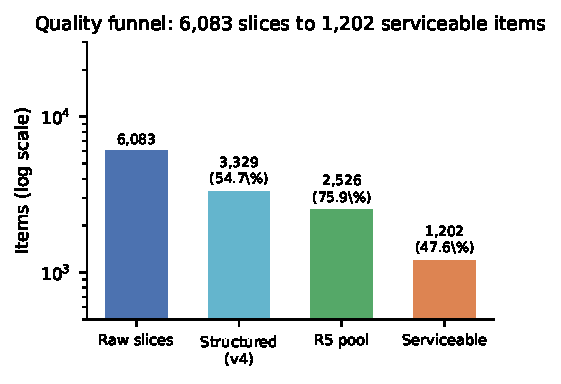
\includegraphics[width=0.62\textwidth]{figures/fig2_funnel.pdf}
\caption{The quality funnel: from 6,083 raw slices of 155 source papers to 1,202 serviceable items. Labels show yields relative to the previous stage.}
\label{fig:funnel}
\end{figure}
\subsection{The QA marathon: 2,526 to 1,202 (47.6\%)}
Figure~\ref{fig:funnel} visualizes the funnel. Ten batches (BATCH6, BATCH8--16; the continuous numbering from BATCH6 has a gap where batch 7 was not archived under that name) audited the recovered pool under one acceptance line: \emph{a student must be able to use the item}. The funnel:

\begin{table}[h]
\centering
\small
\begin{tabular}{lrl}
\toprule
\textbf{Stage} & \textbf{Count} & \textbf{Note} \\
\midrule
Examination papers (ledger) & 155 & distinct \texttt{group\_key}s \\
Raw item slices & 6,083 & \texttt{shanghai\_all.jsonl} \\
Structured items (v4) & 3,329 & unique IDs \\
Usability candidate pool & 2,526 & R5 ledger \\
\textbf{Serviceable (r5\_serve=true)} & \textbf{1,202} & 47.6\% of candidate pool \\
\bottomrule
\end{tabular}
\caption{The quality funnel. A raw-slice to serviceable-item yield of 19.8\%.}
\label{tab:funnel}
\end{table}

Three methodological findings came out of this marathon, each with a concrete incident:

\begin{enumerate}\setlength{\itemsep}{0pt}\setlength{\parskip}{0pt}\setlength{\parsep}{0pt}
\item \textbf{Rendering without crashing $\neq$ item usable.} The first acceptance attempt verified only ``the render pipeline does not throw''; the user review failed it (missing figures, empty answers, broken ions). The usable-item ledger became an on-line gate.
\item \textbf{The auditor must see what students see.}\label{it:auditor-sameness} The screenshot pipeline ran without KaTeX for an entire batch; the vision-language channel judged a different product than the browser. Fix: same-source verification before auditing.
\item \textbf{Precision gold must accompany recall gold.} A new five-dimension reviewer was calibrated only on known-bad items and later misflagged 169 good items in the whitelist ($\approx$13\% of the whitelist). Node-aware text scanning (sentinels for formula/media/omml) fixed it: 0 false positives on 1,207 whitelist rows, and R5 exclusions were re-verified.
\end{enumerate}

Quantified costs: the full-pool vision-language audit of the 2,526 pool cost \textyen17.93; the hardest batch (batch13, ``dead figure'' recovery) rescued 105 assets for \textyen2.53. A P0 hazard was also found and fixed on-line: crop images included printed answers from the original paper, so an OCR answer-leak gate became part of the accept line (Section~\ref{sec:governance}).

\subsection{What the numbers say}
The raw-to-serviceable yield is 19.8\%. This is the \emph{price} of evidence-binding in the data sense: producing a bank where every item's answer is verifiable, its figure is renderable, and its provenance is traceable, costs most of the pool. The 2026-09 file snapshot changed two figures relative to the published white paper (WS2 transcript rows 10,102 and media-ref rows 13,171, vs.\ 6,005 and 12,790 in the earlier report)---a directly measurable consequence of later batch recovery; we report current-tree values as canonical.

\subsection{What is \emph{not} demonstrated}
This pipeline produces a \emph{constructible} bank, not a \emph{validated} one: no student answered any of these items in a controlled setting; no item-difficulty calibration exists beyond the examination's own implicit design; and 926 of 3,329 items lack an \path{answer_source_path} (27.8\%), meaning those items' standard answers rest on the document's answer block alone.

\section{Experiment 1: Can AI Generate Exam Questions? Five Blind Rounds, \textyen13.87}
\label{sec:exp1}

\subsection{Question}
The product needs an ``internalization'' route: instead of reusing the bank, can a generative model write new chemistry items that a student cannot distinguish from examination items? We treated this as a measurement problem, not a capability question, and ran five rounds.

\subsection{Protocol}
Anchor items from the R5 pool; human blind judgments of distinguishability under adversarial pairwise comparison; a cost audit per round; explicit dead/alive verdict per route.

The judge is the author. This is a single-judge protocol, not an expert panel; we state it plainly because it bounds the strength of the finding (Section~\ref{sec:limitations}). The judgment set spans 153 items across three rounds: 60 from-scratch, 53 style-transfer, 40 second-round style-transfer; plus $>$70 figure-anchored items verified by direct inspection. Items were presented in randomized within-pair order; the judge was blind to route and generation round, and only the counting rule (did the judge classify the generated item as real?) was post-hoc. No inter-rater agreement statistic is available by construction; the per-route binomial one-sided 95\% lower bounds are: from-scratch $\geq$77\%, style-transfer $\geq$51\% (60\% fair-condition subset: $\geq$43\%). We report the raw label tables rather than only summary percentages so the reader can recompute.

\begin{table}[h]
\centering
\small
\begin{tabular}{lll}
\toprule
\textbf{Route} & \textbf{Measurement} & \textbf{Verdict} \\
\midrule
From-scratch & 87\% distinguishable & \textbf{dead} (practice only) \\
Style transfer & 65\% / 60\% fair & \textbf{alive} (high-fidelity) \\
Programmatic rendering & passes & live, scalable \\
Figure-anchored reskin & $\approx$26/29 pass & \textbf{alive} \\
\bottomrule
\end{tabular}
\caption{Five-round generation verdicts.}
\label{tab:exp1}
\end{table}

\subsection{Results and the boundary}
From-scratch generation was dead: 87\% of items were distinguishable, twice (two rounds identical), and the marginal gain from a third attempt was measured at zero. Figure~\ref{fig:generation} summarizes the route-level measurements. Style transfer survived: 65\% distinguishable under adversarial comparison, 60\% under fair conditions---still above chance, but a real working band. The product rule that followed: \emph{generated items never enter the diagnostic path}.

\begin{figure}[t]
\centering
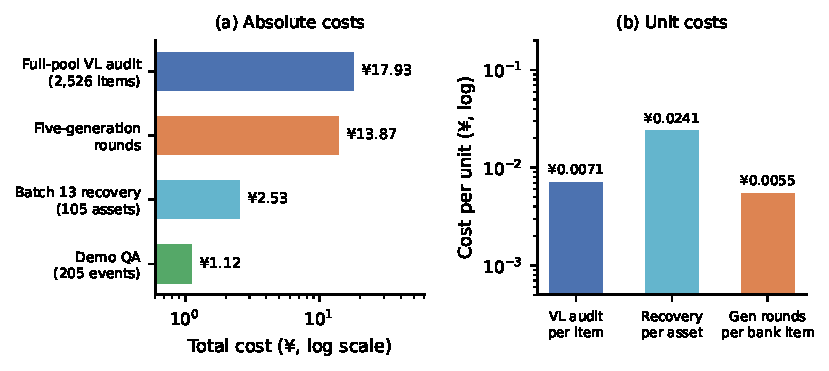
\includegraphics[width=\textwidth]{figures/fig6_costs.pdf}
\caption{Measured costs of the evidence pipeline: absolute (a) and per-unit (b). Note the log scales.}
\label{fig:costs}
\end{figure}

\begin{figure}[t]
\centering
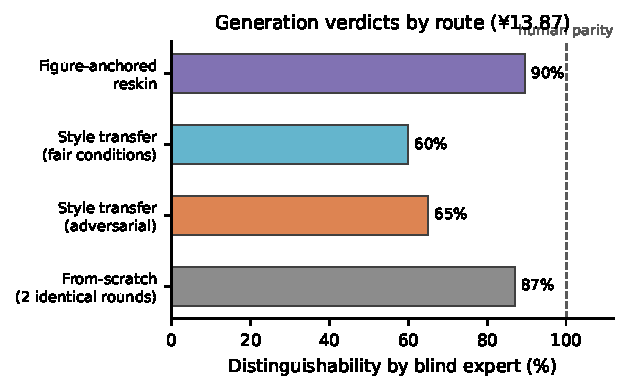
\includegraphics[width=0.6\textwidth]{figures/fig3_generation.pdf}
\caption{Five-round generation verdicts. Distinguishability by blind expert under adversarial pairwise comparison. The dashed line marks human parity.}
\label{fig:generation}
\end{figure}



Figure~\ref{fig:costs} places the audit costs in context. The five rounds cost \textyen13.87 in total; this is API and tooling spend, not compensated human review---the blind judgments were contributed by the author without payment.

\subsection{Why this matters for the genre}
Three meta-lessons, each recorded as a product rule:
\begin{enumerate}\setlength{\itemsep}{0pt}\setlength{\parskip}{0pt}\setlength{\parsep}{0pt}
\item \textbf{Adversarial distinguishability is not student-scenario serviceability.} A generated item can be both more distinguishable and more usable than a real item; these are different orders.
\item \textbf{Generators inherit the corpus's transcription scars.} When the reference bank itself has residual defects (ion subscripts, figures), generation reproduces them and adds new ones.
\item \textbf{Goodhart is a property of any acceptance rule.} Every acceptance line must anchor to non-forgeable concrete objects---numeric values, IDs, hashes---never to semantic interpretation.
\end{enumerate}

\subsection{Against the literature}
Published blinded evaluations of AI-generated multiple-choice items often find judges perform at or near chance (51.4\% source identification in \cite{nursing2025}; 69.2\% and 73.6\% of participant ratings for the two highlighted exercise questions wrongly rated as Human in \cite{chatgptqg2025}; blinded medical panels rating GPT-4 items comparable to expert human items in overall impression, with higher rates of items unfit for use \cite{medicalteacher2025}); under item-response-theory analysis, prompted generation can produce items with human-like difficulty and discrimination \cite{anaquest2025}. Our 87\%/65\% numbers are higher. We attribute this to (a) examination-specific fidelity of the reference set (real Shanghai items have distinctive surface signatures: multi-step compound reasoning, figure-anchored stems, standardized answer keys) and (b) the private gold-label protocol that governs ours. We do not generalize: this is a measurement on one examination system.

\section{Experiment 2: Three-Round Architecture Audit}
\label{sec:exp2}

\subsection{Design}
Three rounds, each with a distinct epistemic function:
\begin{enumerate}\setlength{\itemsep}{0pt}\setlength{\parskip}{0pt}\setlength{\parsep}{0pt}
\item \textbf{Round 1 (component-wise adjudication).} 21 engine components enumerated; each adjudicated against the state of the art.
\item \textbf{Round 2 (independent re-review).} 47 claims re-examined by a second reviewer; 30 REVISE / 5 REPLACE, overturning several prior numbers. ``Independent'' here means independent \emph{within the audit pipeline} (a separate reviewer persona executing against a frozen evidence set, with no access to the prior round's conclusions until after independent adjudication); it does not mean external review by third-party scholars, and we do not claim that.
\item \textbf{Round 3 (literature + adversarial).} Six literature lanes (arXiv/Crossref/ERIC) plus three red-team attack passes plus one independent verification round.
\end{enumerate}

\subsection{Quantified findings}

Figure~\ref{fig:auditnums} plots the measurements that survived re-verification.

\begin{figure}[t]
\centering
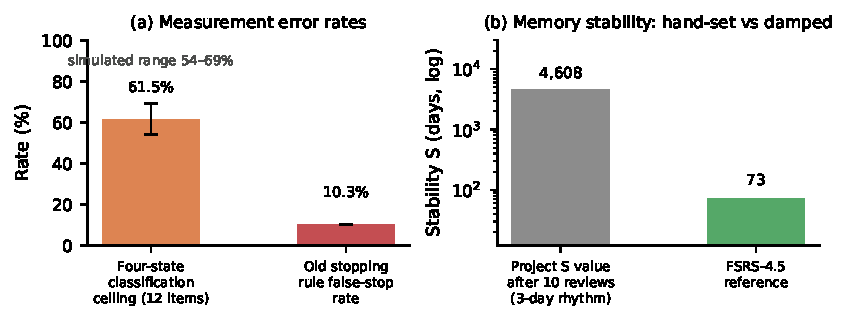
\includegraphics[width=\textwidth]{figures/fig5_audit_numbers.pdf}
\caption{The hardest audit numbers. (a) Measurement error rates with simulation range; (b) memory stability: the hand-set formula produced S=4,608~d vs.\ the FSRS-4.5 reference of 73~d after 10 reviews at a 3-day rhythm.}
\label{fig:auditnums}
\end{figure}

\begin{table}[h]
\centering
\small
\begin{tabular}{@{}p{6.4cm}p{3.2cm}p{4.0cm}@{}}
\toprule
\textbf{Finding} & \textbf{Value} & \textbf{Source} \\
\midrule
Four-state classification accuracy after 12 items & 54--69\% (two sim. runs) & redteam 1 \\
P/U non-identifiability & KL = 0.0247 & lane 1; redteam 1 \\
Old stopping (gap $>$ 0.45) false-stop & 10.3\% & redteam 1 \\
FSRS hand-set multipliers, 10 reviews & S = 4,608 d (4.5: 73) & redteam 2; round 4 \\
n=2 held-out one-sided 95\% CI & 22.4\% & round 4 \\
SymPy \texttt{simplify} false equivalences & 7 / 5 reproduced & redteam 3 \\
\bottomrule
\end{tabular}
\caption{The hardest numbers, each traced to the report that produced it. The four-state ceiling is reported as the range across two independent simulation runs (master audit, 2026-08-13); the individual runs in redteam 1 produced 4-way accuracy 61.4\% and 61.1\% at 12 items.}
\label{tab:exp2}
\end{table}

\begin{figure}[t]
\centering
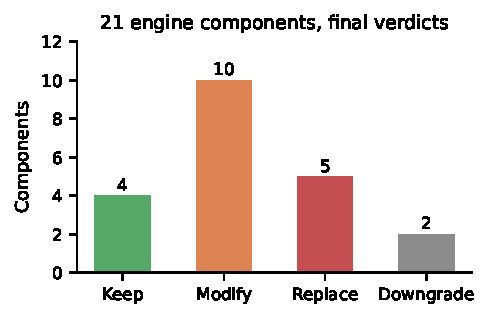
\includegraphics[width=0.55\textwidth]{figures/fig4_audit_verdicts.pdf}
\caption{Final verdicts across the 21 audited engine components.}
\label{fig:verdicts}
\end{figure}
\subsection{Verdicts}
Figure~\ref{fig:verdicts} shows the distribution. Across 21 components: \textbf{4 keep / 10 modify / 5 replace / 2 downgrade} (\texttt{docs/audit-history/MASTER\_AUDIT\_REPORT\_2026-08-13.md}, verified against the frozen evidence matrix of 47 claims: 30 REVISE / 5 REPLACE / 7 EXPERIMENT\_ONLY / 4 UNKNOWN / 1 RETIRE). The final column: inference keeps binary mastery + prerequisite prior + error-code routing (four UI labels retained); stopping becomes P(top1) $\geq$ 0.8 with min\_length 4--5 with gap display-only; memory switches to the FSRS-4.5 damped formula; efficacy score is demoted to a tie-break (5pp real difference at n=20 still flips 30\% of replicates); held-out early-stop protocol becomes 3$\rightarrow$6, never n=2 binary; events gain a provenance field (source $\in$ \{real, qa, synthetic\}).

\subsection{Drop-in changes already in the tree}
Three verdicts are implemented and tested: FSRS-4.5 damped stability with $S_{\max}=500$~d; stopping on P(top1)$\ge$0.80 with min direct answers 4; event provenance with schema\_version 2. Each has regression tests in \texttt{tests/}.

\subsection{What this audit does and does not prove}
It proves that the engine's \emph{design assumptions} are individually checkable, and that three of them were wrong in measurable ways. It does not prove the engine works on students.

\section{Engineering Governance: The Off-by-One That Cost a Day}
\label{sec:governance}

The project's history includes two incidents that are themselves evidence---they show what happens when an acceptance rule is not anchored to concrete, non-forgeable objects, and what happened when it was.

\begin{enumerate}\setlength{\itemsep}{0pt}\setlength{\parskip}{0pt}\setlength{\parsep}{0pt}
\item \textbf{2026-06-28, agent-loop incident.} An autonomous agent loop issued 1,418 tool calls and leaked a plaintext API key into a log. The countermeasure was not a bigger model; it was a governance discipline: signed review, contract-based authorization, and a secrets rule (no plaintext keys in tracked files).
\item \textbf{2026-07-03, P0 answer-leakage.} Cropped images for visual items included printed answers from the original paper; the item-shaping pipeline had copied the printed region. This is why an OCR answer-leak gate became an on-line check, and why the pipeline now verifies answer blocks separately from stems.
\item \textbf{2026-07-13, governance flip.} Contract-based authorization (unsigned reviewer claims) was replaced by the \emph{reversibility discipline}: every write to official data requires (a) a ``\texttt{\_backup\_pre\_<step>\_<date>}'' backup and (b) a line-by-line change manifest, single-command rollback; backups are never deleted. The reviewer may sign (reviewer=codex/claude, dated, with evidence), but the user remains the only authority for irreversible, outward-facing actions.
\item \textbf{2026-07-17, double gate for research deliverables.} After a review deliverable that was perfectly honest and contributed nothing, two gates became mandatory for any research artifact: an \emph{honesty gate} (is every claim true?) and a \emph{contribution gate} (does it matter?). The present manuscript is the first document produced under both gates.
\end{enumerate}

Each audit report in \path{docs/audit-history/} lists exact commands, input hashes, and verdict tables; where a verdict was overturned later (Section~\ref{sec:exp2}), the overturn is itself recorded.

\section{Limitations}
\label{sec:limitations}

This manuscript is an engineering-evidence report; the following limitations are therefore not afterthoughts but the frame in which every claim should be read.

\begin{enumerate}\setlength{\itemsep}{0pt}\setlength{\parskip}{0pt}\setlength{\parsep}{0pt}
\item \textbf{No real students.} All conclusions are simulation-, audit-, or engineer-derived. There is no retention, learning-effect, or usability evidence from actual learners. The system's learning loop is \emph{designed}, not \emph{validated}.
\item \textbf{Simulated counterexamples rest on synthetic parameters and hand-set constants.} Directional conclusions are robust; point estimates are not calibrated. Where a red-team number says ``54--69\% classification ceiling,'' it is a property of the simulation's assumptions, not a property of students.
\item \textbf{The chemistry line is frozen.} The engine is a design audited but not modified per verdicts---the 10 modify / 5 replace items are each documented with a specific fix, but not yet applied (except the 2026-09 drop-in changes: FSRS-4.5 damping, P(top1) stopping, provenance field, each with regression tests).
\item \textbf{Document-level provenance gaps.} 926 of 3,329 items (27.8\%) lack an \texttt{answer\_source\_path}; those items' answers rest on the single document's answer block, not on a separately sourced answer key.
\item \textbf{Item-bank copyright boundary.} Items come from public examination papers; this is a mechanical restructuring of exam content, not original creation. The repository's data layers are released under CC BY-NC to make the boundary explicit (code: MIT).
\item \textbf{Chinese-language assessment literature unreachable.} CNKI/Wanfang were blocked during the review; the Chinese assessment tradition is represented at metadata level only.
\item \textbf{Supplier survivor bias.} In an earlier exploratory persona-collection exercise, three of six LLM providers failed collection and were excluded (documented); any conclusions drawn from the remaining three are subject to survivor bias.
\item \textbf{The system was built and audited by a small team with AI assistance.} This is disclosed fully in the back matter; it is a strength in engineering discipline and a limitation in independence.
\end{enumerate}

\section{Reproducibility}
\label{sec:repro}

\begin{itemize}\setlength{\itemsep}{0pt}\setlength{\parskip}{0pt}\setlength{\parsep}{0pt}
\item \textbf{Artifacts}: \path{github.com/Chris-TLC/YHer-skill} (public), plus an HF dataset mirror \path{Chris-TLC/yher-chemistry-question-bank} with a deterministic builder (\path{scripts/make\_hf\_dataset.py}).
\item \textbf{Data}: \texttt{data/README.md} documents schema, R5 definition, and license.
\item \textbf{Session reconstruction}: single-node deterministic path (\texttt{YHER\_ENABLE\_PAID\_LLM=0}), synthetic-replay corpus under \texttt{SYNTHETIC\_DEMO}, no cross-contamination with real or QA events.
\item \textbf{Audits}: every number in this paper is traceable to \texttt{docs/audit-}\texttt{history/}, which records exact commands, input hashes, and verdict tables.
\end{itemize}

Reproduction instructions at the command level are provided in Appendix~\ref{app:commands}; they have been run in a clean checkout as part of the audit workflow reported here.

\section{Related Work}
\label{sec:related}

\begin{itemize}\setlength{\itemsep}{0pt}\setlength{\parskip}{0pt}\setlength{\parsep}{0pt}
\item \textbf{Knowledge tracing.} Corbett and Anderson's Bayesian Knowledge Tracing \cite{corbett1995}, Yudelson et al.'s individualized BKT \cite{yudelson2013}, Piech et al.'s Deep Knowledge Tracing \cite{piech2015}, and graph-based variants \cite{nakagawa2019}. Our belief model is a four-state extension of BKT's two-state assumptions, with prerequisite structure---the closest published analogue is Zhang and Yao's three-state BKT \cite{zhang2018}.
\item \textbf{Item response theory and adaptive testing.} Rasch's original model \cite{rasch1960}, Embretson and Reise \cite{embretson2000}, and CAT item selection and exposure control \cite{vanderlinden1999, eggen2014, sorrel2020, mao2013}. Our EIG selector is a Bayesian information-gain rule within a cognitive-diagnosis frame; CAT exposure control informed our seen-exclusion rule.
\item \textbf{Spaced repetition and memory models.} The stochastic shortest path formulation of FSRS-4.5 \cite{ye2022}, LSTM-based spacing models \cite{pokrywka2023}, spacing schedule experiments \cite{kang2014}, and trainable spaced repetition models for language learning \cite{settles2016}. Our audit of the memory module applied the FSRS-4.5 damping formula as the reference implementation.
\item \textbf{LLMs in education.} Recent work combines LLMs with tutoring-system intelligence \cite{tutorLLM2024}, applies LLM prompting to knowledge tracing over tutor-student dialogue \cite{llmkt2025}, and reports expert judges frequently \emph{cannot} distinguish LLM-generated multiple-choice items above chance \cite{anaquest2025, chatgptqg2025, medicalteacher2025}. Our finding (65\% distinguishability, adversarial) stands in contrast to that literature's aggregate; we attribute the difference to the examination-specific fidelity of the reference items and to the private, domain-blind gold-label protocol, and we do not generalize beyond chemistry.
\item \textbf{LLM capabilities and system building blocks.} Verifier training \cite{cobbe2021} and the GPT-4 capability report \cite{gpt4} frame what the product \emph{does not} delegate to generative AI: new chemistry facts and standard answers.
\end{itemize}


\bibliographystyle{plain}
\bibliography{references}

\section{Conclusion}

We built a diagnostic learning loop whose central property is evidence-binding: every conclusion traceable, every answer sourced, every recommendation signed. We measured the cost of that property in the data pipeline (6,083 raw slices $\rightarrow$ 1,202 serviceable items, 19.8\%), in the generation boundary (from-scratch generation dead at 87\% distinguishability; style transfer alive at 65\%), and in the engine's own audit (4 keep / 10 modify / 5 replace / 2 downgrade across 21 components, with the hardest numbers quantified). We did not---and cannot, from the evidence in hand---claim any effect on student outcomes.

The next step is the one step this report deliberately does not take: a pre-registered pilot with real learners, which this manuscript treats as the plan it is designed to serve.

\section*{Author Contribution and AI-Authoring Statement}

\textbf{Author contributions.} The author of this manuscript designed and directed the engineering effort (including the reversibility governance flip), made all product decisions, and conducted the end-to-end curation and acceptance review. Assistant systems contributed design proposals, implementation, and audits under an explicit signed-review protocol (reviewer=claude or codex, with dates and evidence).

\textbf{AI usage disclosure.} Claude and Codex assisted with implementation, audit execution, and manuscript drafting. Factual claims, data points, and citations in this manuscript were checked against the repository and audit records, with a dedicated independent verification pass; that pass found and corrected two quantitative statements and seven bibliographic entries, and its report accompanies this manuscript.

\section*{Acknowledgements}
The author thanks the system-design and audit assistant systems for the proposal and verification labor that made the engineering evidence possible. The item bank originates from publicly released Shanghai chemistry examinations; the remainder of this report stands on the audit records in \texttt{docs/audit-history/}.

\appendix
\section{Reproduction Commands}
\label{app:commands}

All commands below were run at the repository state reported here (public tree, main branch). The item-bank rebuild, test suite, and demo boot do not require any paid API: the deterministic path uses \texttt{YHER\_ENABLE\_PAID\_LLM=0}.

\begin{enumerate}\setlength{\itemsep}{0pt}\setlength{\parskip}{0pt}\setlength{\parsep}{0pt}
\item \textbf{Clone and install.}
\small
\begin{verbatim}
git clone https://github.com/Chris-TLC/YHer-skill.git
cd YHer-skill
python3 -m venv .venv-pub
.venv-pub/bin/pip install -r requirements-dev.txt
YHER_ENABLE_PAID_LLM=0 ./deploy/run_demo.sh   # self-bootstraps .venv-demo, port 8700
\end{verbatim}
\item \textbf{Health check.}
\small
\small
\begin{verbatim}
curl -fsS http://127.0.0.1:8700/health | python3 -m json.tool
\end{verbatim}
\item \textbf{Re-derive the audit-critical counts} (item IDs, R5 ledger, media map):
\small
\small
\begin{verbatim}
wc -l data/item_bank/v4/chemistry_v4_1_3329.jsonl   # 3329 items
wc -l data/item_bank/v4/usability_r5_v1.jsonl      # 2526 R5 ledger rows
python3 -c "import json
print(sum(1 for l in open('data/item_bank/v4/usability_r5_v1.jsonl')
          if json.loads(l).get('r5_serve') in (True,'True')))"   # 1202 serviceable
\end{verbatim}
\item \textbf{Build the Hugging Face mirror} (deterministic):
\small
\small
\begin{verbatim}
python3 scripts/make_hf_dataset.py --sample-only          # local sample (55 items)
python3 scripts/make_hf_dataset.py --push <dataset-id>    # full push, needs HF token
\end{verbatim}
\item \textbf{Run the regression suite} (engine-default config; paid tests excluded; the mark filter comes from \texttt{pytest.ini}):
\small
\begin{verbatim}
PYTHONDONTWRITEBYTECODE=1 .venv-pub/bin/python -B -m pytest -q --timeout=120
\end{verbatim}
\item \textbf{Deterministic session replay} (synthetic corpus):
\small
\small
\begin{verbatim}
YHER_ENABLE_PAID_LLM=0 ./deploy/run_demo.sh \
  # synthetic material under demo/synthetic_scenarios/, SYNTHETIC_DEMO label
\end{verbatim}
\end{enumerate}

Every audit report in \texttt{docs/audit-history/} lists the exact commands, input hashes, and verdict tables for the numbers quoted in this manuscript; the audit history index (\texttt{docs/audit-history/README.md}) maps each claim in this paper to its report.


\end{document}
